\section{Non-functional Resource Sharing}


As explain before two or more operation can be bound to the same resource. Before we bond them together we need to ensure that they are \textit{compatible}. Two conditions that the operations should met in order to be \textit{compatible} :

\begin{itemize}
\item The operations is not concurrent.
\item The operations can be implemented by resources of the same type.
\end{itemize}

So, $ E+\{(v_{i},v_{j})|\tau(v_{i}=v_{j} $ and $ ((t_{i}=d_{i} \leq t_{j}) $ or $ t_{j}=d{j} \leq t_{i})),i,j=1,...,n_{ops}\}$ %


\subsection{Register Sharing}

We consider in this section those registers that hold the values of the variables. Recall that each variable has a lifetime that is the interval from its birth to its death, where 
the former is the time at which the value is generated as an output of an operation and the latter is the latest time at which the variable is referenced as an input to another operation. We assume that those variables with multiple assignments within one model are aliased, so that each variable has a single lifetime interval in the frame of reference corresponding to the sequencing graph entity where it is used. Note that the lifetimes can be data dependent, for example, due to branching and iterative constructs.

Whereas an implementation that associates a register with each variable suffices, it is obviously inefficient. Indeed, variables that are alive in different intervals or under alternative conditions can share the same register. Such variables are called compatible. The register compatibility and conflict graphs are defined analogously to the resource compatibility and conflict graphs. The problem of minimizing the number of registers can be cast in a minimum clique partitioning problem of,the compatibility graph or into a minimum coloring problem of the conflict graph. We consider now how these graphs are generated and their properties. Let us consider first non-hierarchical sequencing graphs. In this model, a conflict between two variables corresponds to a lifetime overlap. Since in this model the variable lifetimes are intervals, the conflict graph is 'an interval graph and its complement is a comparability graph. Therefore, optimum register sharing can be computed in polynomial time.

Consider just a portion of the sequencing graph of Figure \ref{Scheduled_sequencing_graph}, shown in Figure \ref{fig:Sequencing_graph_fragment}(a). There are six intermediate variables, named $ \{z_{i},i=1,2,...,6\} $, that must be stored in registers. The lifetime of three pairs of these variables is conflicting, as shown by the conflict graph in Figure \ref{fig:Sequencing_graph_fragment}(c). These variables can be implemented by two registers, which is the chromatic number of the conflict graph.


Let us now consider sequencing models of iterative bodies. In this case, some variables are alive across the iteration boundary, for example, the loop-counter variable. The cyclicity of the lifetimes is modeled accurately by circular-arc graphs that represent the intersection of arcs on a circle. We consider the full differential equation integrator. There are 7 intermediate variables $ \{z_{i},i=1,2,...,6\} $, 3 loop variables $ \{x,y,z\} $ and 3 loop invariants  $ \{a,3,dx\} $. We consider here the intermediate and loop variables and their assignment to registers. The data-flow graph is shown in Figure \ref{fig:Sequencing_graph}(a) along with the explicit annotation of the variables. The variable lifetimes are shown in Figure  \ref{fig:Sequencing_graph}((b) and are represented as arcs on a circle in Figure \ref{Variable_lifetimes_as_arcs_on_a_circle}. The corresponding circular-arc conflict graph is shown in Figure \ref{fig:Circular_arc_confliCr_graph}. Five registers suffice to store the 10 intermediate and loop variables. 

The register sharing problem can then be cast as a minimum coloring of a circular-arc graph that unfortunately is intractable. Stok [??] has shown that this problem can be transformed into a multi-commodity flow problem and then solved by a primal algorithm.

Register is used by a circuit to store values of variable. Since variable have life time it can be interval. This variable value will be use letter by other operation as an input.
\ref{fig:Sequencing_graph_fragment}
\begin{figure}[h]
    \centering
    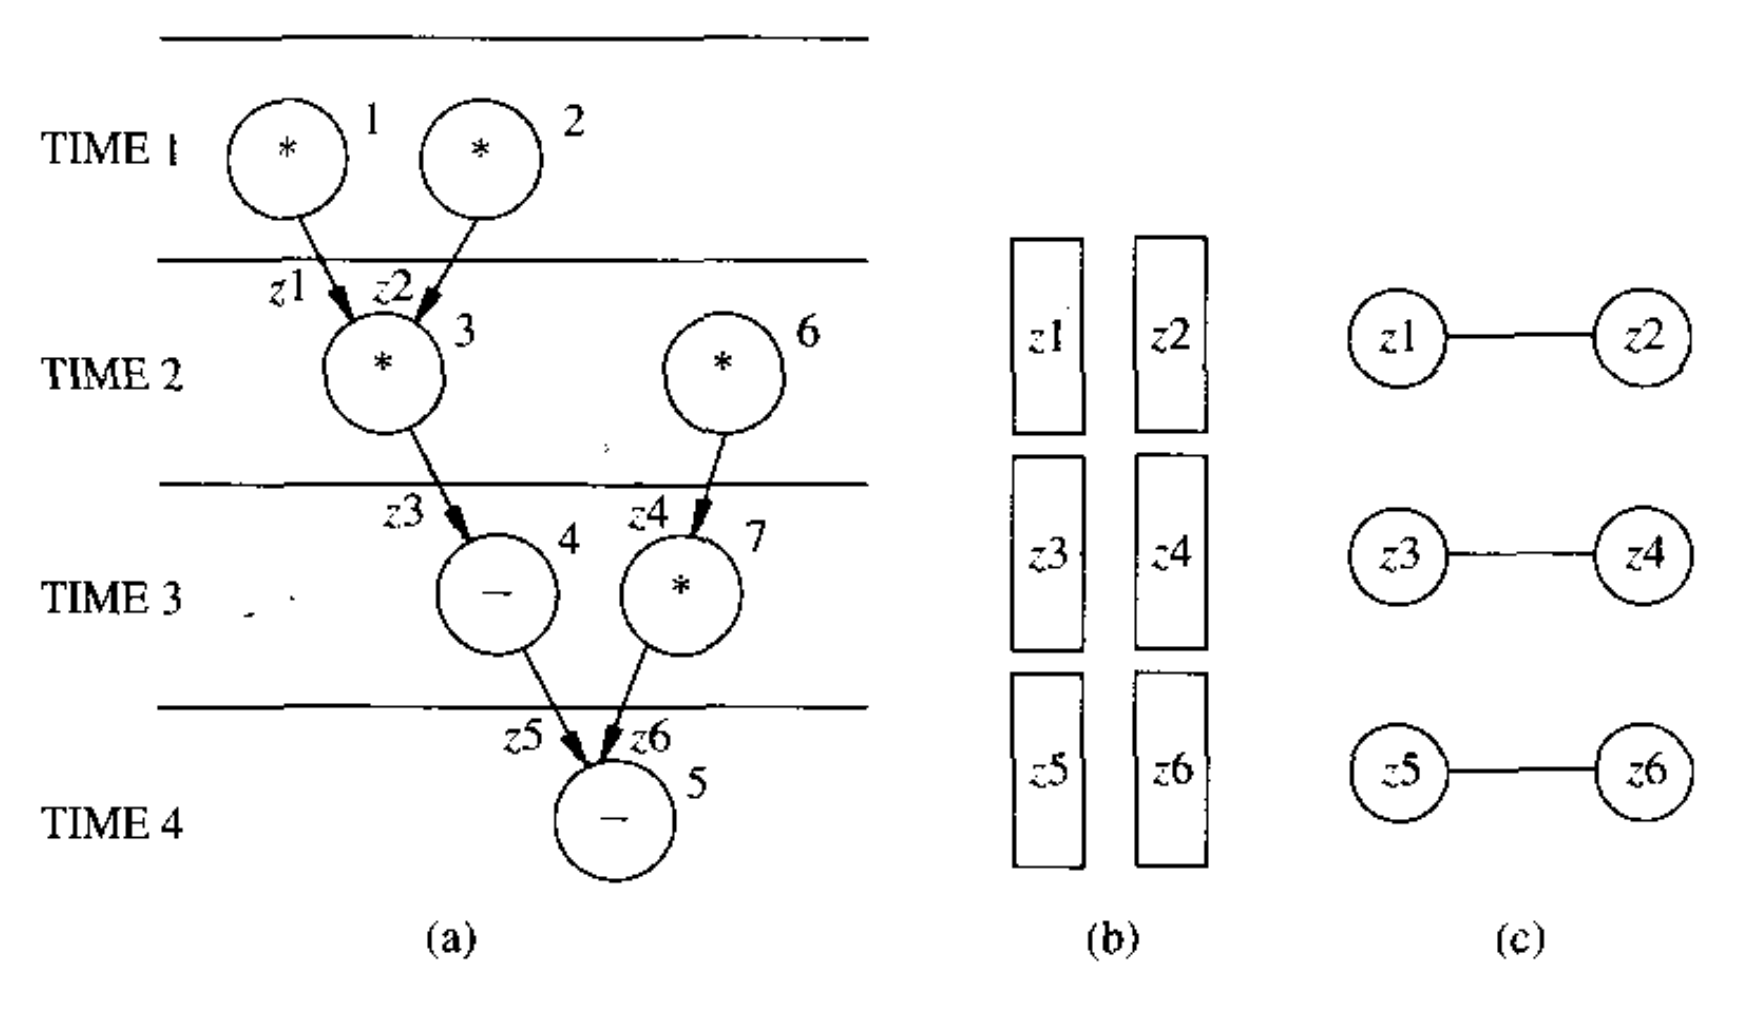
\includegraphics[width=0.5\textwidth]{Sequencing_graph_fragment}
    \caption{ a) Sequencing graph fragment. (b) Variable intervals. (c) Conflict mph \cite{b1}}
    \label{fig:Sequencing_graph_fragment}
\end{figure}

\ref{fig:Sequencing_graph}
\begin{figure}[h]
    \centering
    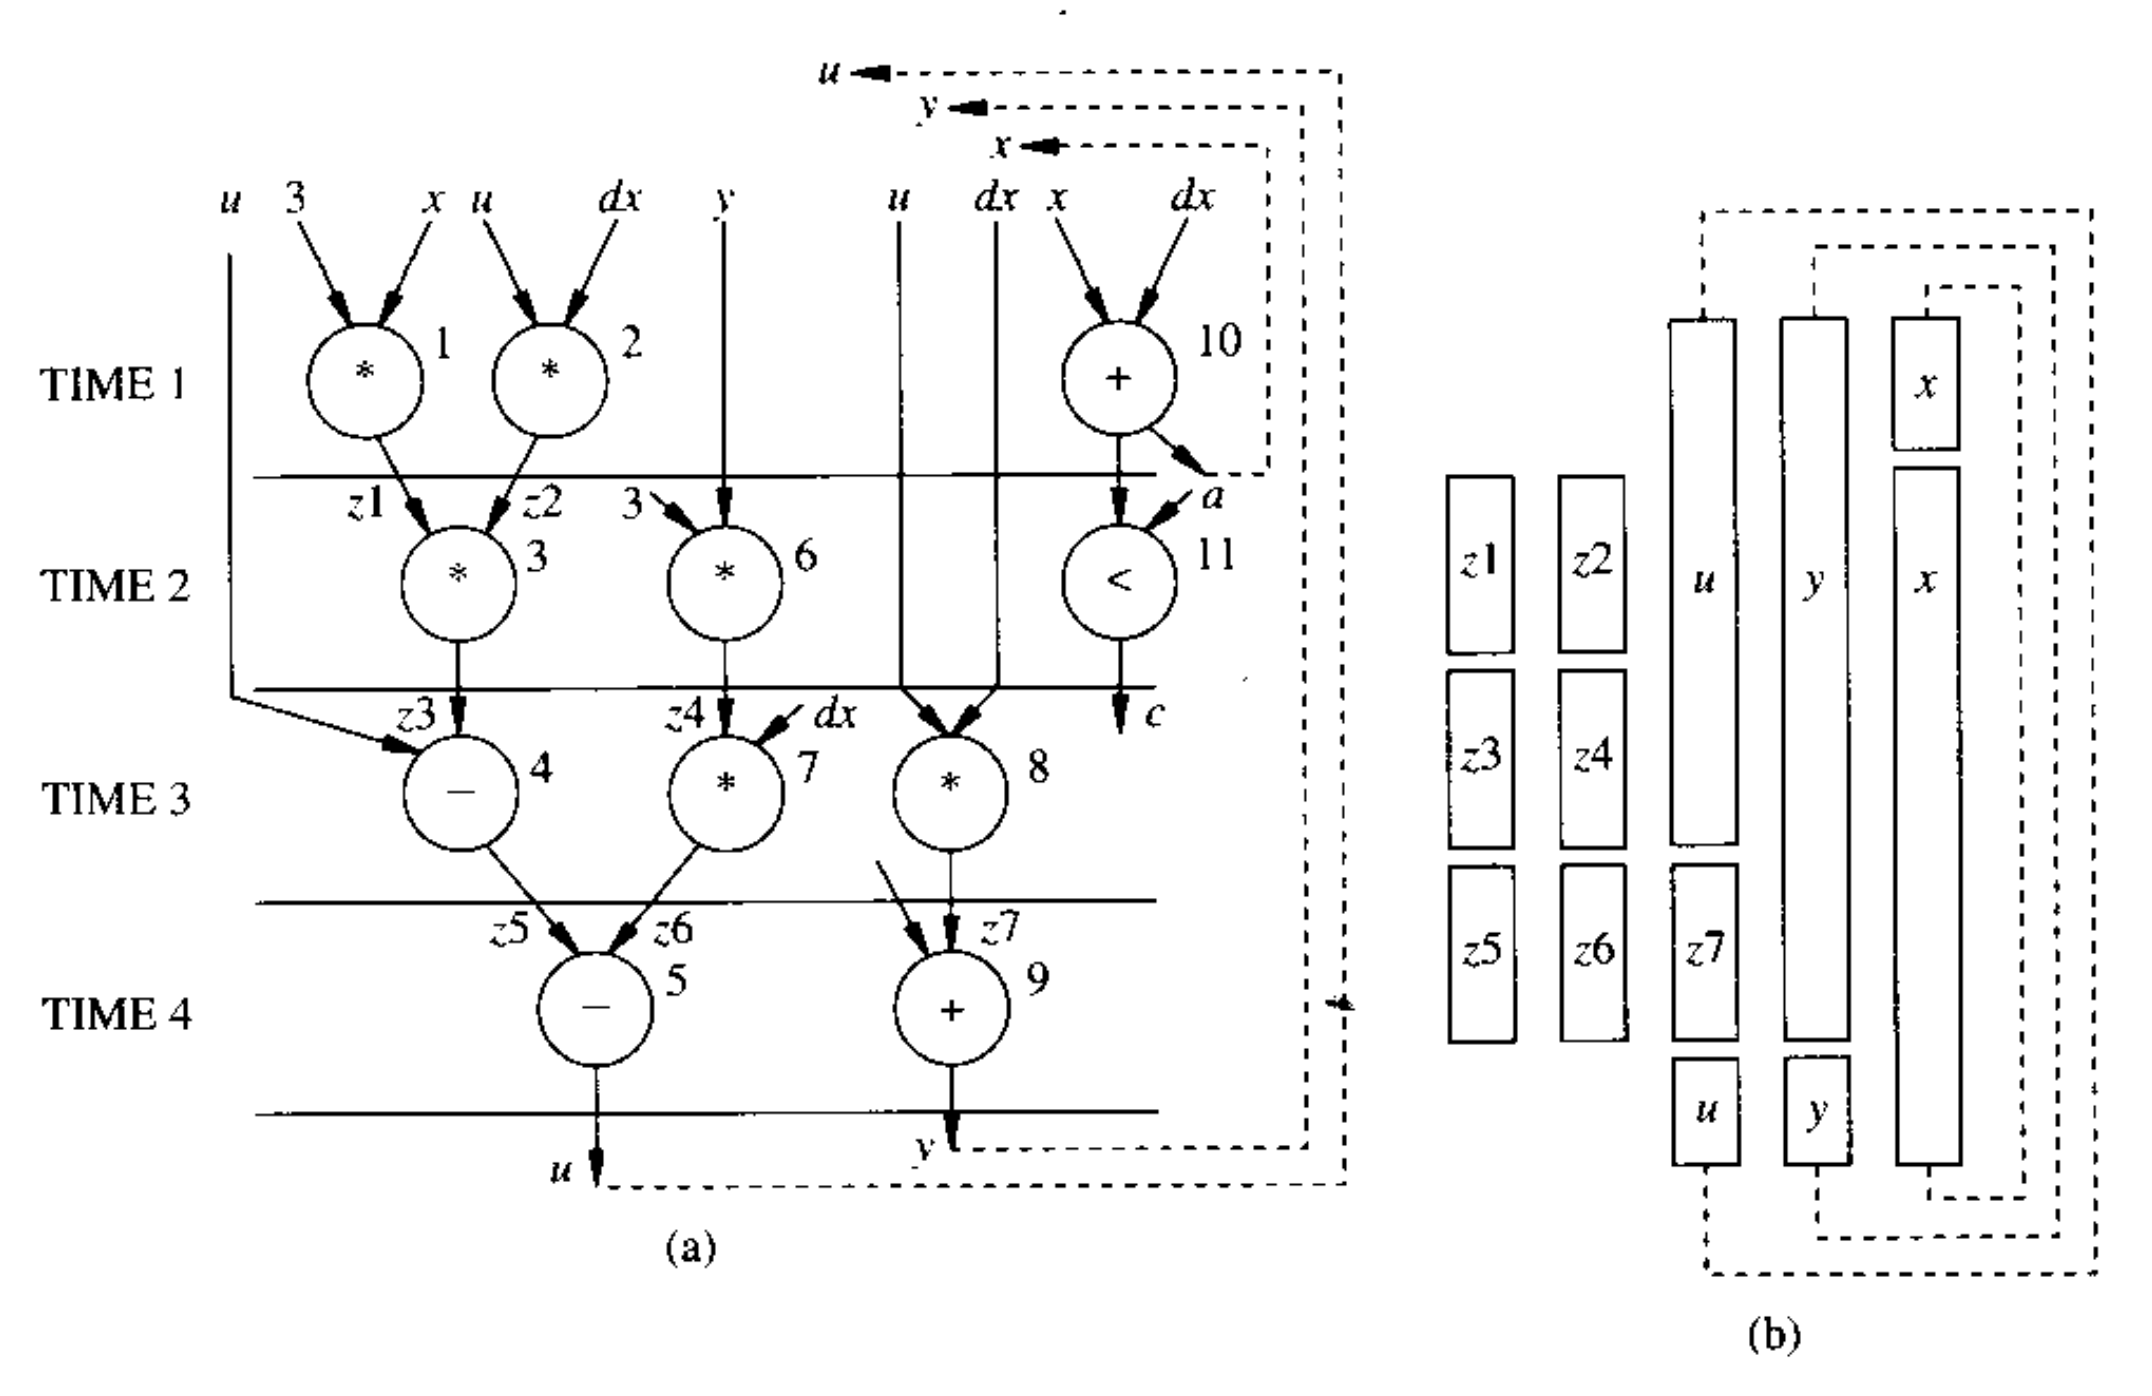
\includegraphics[width=0.5\textwidth]{Sequencing_graph}
    \caption{ (a) Sequencing graph. (b) Variable lifetimes \cite{b1}}
    \label{fig:Sequencing_graph}
\end{figure}

\ref{fig:Variable_lifetimes_as_arcs_on_a_circle}
\begin{figure}[h]
    \centering
    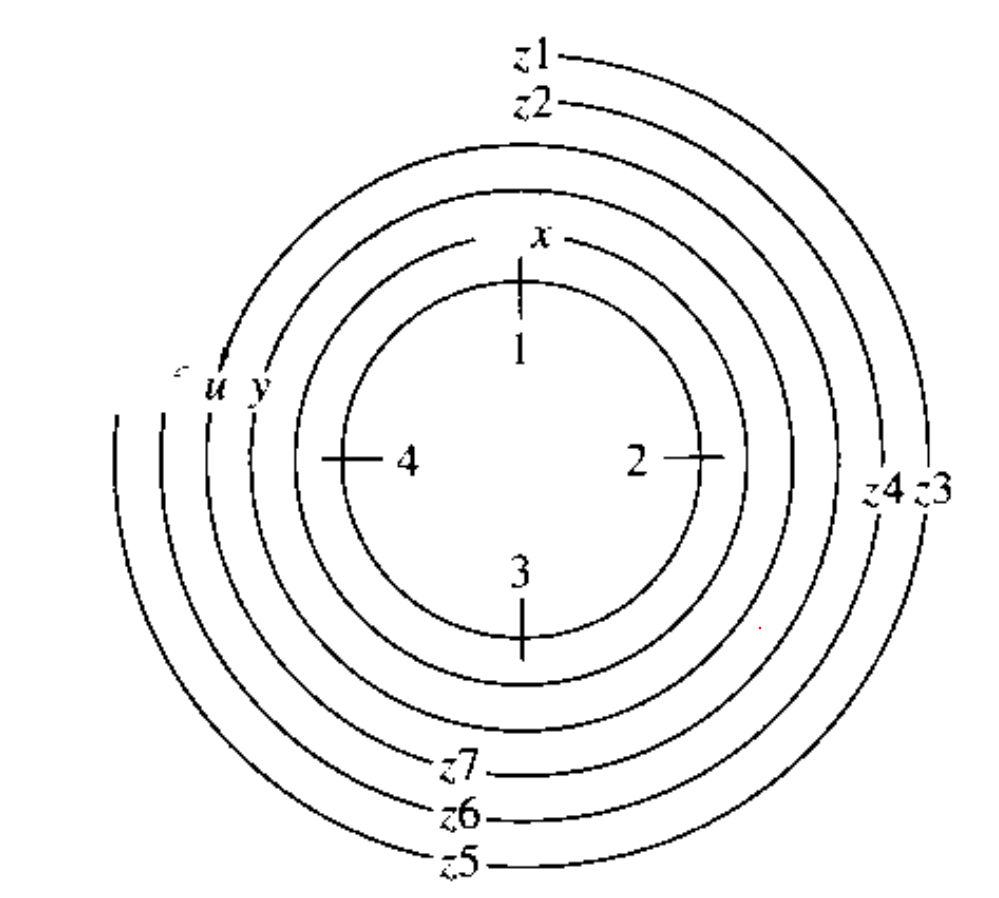
\includegraphics[width=0.4\textwidth]{Variable_lifetimes_as_arcs_on_a_circle}
    \caption{ Variable lifetimes as arcs on a circle \cite{b1}}
    \label{fig:Variable_lifetimes_as_arcs_on_a_circle}
\end{figure}

\ref{fig:Circular_arc_confliCr_graph}
\begin{figure}[h]
    \centering
    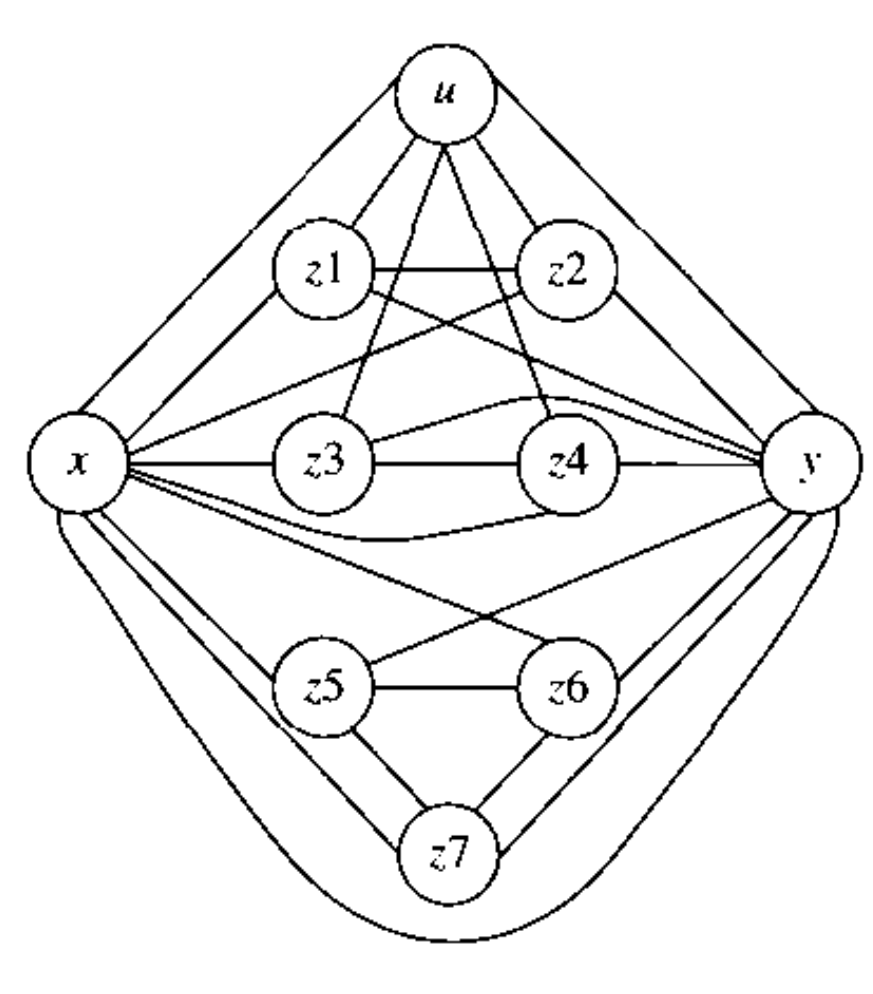
\includegraphics[width=0.4\textwidth]{Circular_arc_confliCr_graph}
    \caption{ Circular-arc conflict graph \cite{b1}}
    \label{fig:Circular_arc_confliCr_graph}
\end{figure}

The register sharing problem can be extended to cope with hierarchical models. The register compatibility and conflict graphs can be derived by traversing the hierarchy and comparing the variable lifetimes. The properties of these graphs depend on the structure of the hierarchy, as in the case of the resource compatibility and conflict graphs. In particular, interval conflict graphs can be derived from hierarchical models with only single model calls by considering the variable lifetimes with reference to the start time of the sequencing graph entity in the root model of the hierarchy. In the general case. register compatibility and conflict graphs may not have any special property, and therefore the corresponding optimum register sharing problem is intractable. 

Springer and Thomas [??] have shown that polynomial-time colorable conflict graphs can be achieved by enforcing some restrictions on the model calls and on the branch types. The register sharing problem can be formulated by ILP constraints, mutaris murandis, similarly to the resource sharing problem. 

\subsection{Multiple Memory Binding}
We consider now the problem of using multi-port memory arrays to store the values of the variables. Let us assume a memory with a ports for either read or write requiring one cycle per access. Such a memory array can be a general purpose register file common to RISC architectures. We assume the memory to be large enough to hold all data. We consider in this section non-hierarchical sequencing graphs; extensions are straightforward and similar to those presented in the previous sections. 
A first problem corresponds to computing the minimum number of ports a required to access as many variables as needed. If each variable accesses the memory always through the same port, then the problem reduces to binding variables to ports. Thus the considerations for functional resource binding can be applied to the ports, which can be seen as interface resources. 

On the other hand, if the variables can access the memory array through any port,the minimum number of ports is equal to $\underset{1\leq l \leq \lambda + 1}{\mathrm{max} \sum_{i=1}^{n_{var}} x_{il}} $ is the total number $ {n_{var}} $ of variables and X is a set of binary constants determined by scheduling, where $ x_{il} $ is 1 when the access of variable $ i,i=1,2,...,n_{var} $ is at step $ l,l=1,2,..., \lambda+1 $. In other words, the maximum number of concurrent accesses is the minimum number of ports. 
Balakrishnan et al. [??] considered the dual problem. They assumed a fixed number of ports and maximized the number of variables to be stored in the multi-port memory array, subject to the port limitation. They formulated the problem as follows. 
Let $ b \in \{0,1\}^n_{var} $  be a binary-valued vector whose entries denote whether the corresponding variable is stored in the array or not. Let $ \mathds{1} $ be a $ n_{var}  $ dimensional vector of all 1s. Then the desired variables are indicated by a solution to:

\begin{center}
$\mathds{1}^{T} b = \sum_{i=l}^{n_{var}}b_{i}$
\end{center}

\begin{equation}\label{1b}
sun_{i=l}^{n_{var}}b_{i}x_{il} \leq a \; l=1,2,..., \lambda +1 
\end{equation}

This problem can be extended easily to handle separate read and write ports and to the interconnect minimization problem [??]. 
This example is borrowed from reference [2]. Consider the following scheduled sequence of operations, which requires the storage of variables $ \{z_{i}, i =1,2,...,15\} $ 


$time-step \; 1:\; z_{3}=z_{1}+z_{2};z_{12}=z_{1}$

$time-step \; 2:\; z_{5}=z_{3}+z_{4};z_{7}=z_{3}*z_{6};z_{13}=z_{3}$

$time-step \; 3:\; z_{8}=z_{3}+z_{5};z_{9}=z_{1}*z_{7};z_{11}=z_{10}/z_{5}$

$time-step \; 4:\; z_{14}=z_{11}\wedge z_{8};z_{15}=z_{12}\vee z_{9}$

$time-step \; 5:\; z_{1}=z_{14};z_{2}=z_{15}=z_{3}$


Let us consider a memory array with a ports. Then, the problem can be represented by maximizing $  sum_{1=1}^{15} b_{i}$ under the following set of constraints: 

\begin{flushright}
$ b_{1}+b_{2}+b_{3}+b_{12}\leq a $

$ b_{3}+b_{4}+b_{5}+b_{6}+b_{7}+b_{13}\leq a $

$ b_{1}+b_{3}+b_{5}+b_{7}+b_{8}+b_{9}+b_{10}+b_{11}\leq a $

$ b_{8}+b_{9}+b_{11}+b_{12}+b_{14}+b_{15}\leq a $

$ b_{1}+b_{2}+b_{14}+b_{15}\leq a $
\end{flushright}


This problem with a one-port memory (i.e., $ a = 1 $) yields a solution where only $ \{b_{2},b_{4}b_{8} \}$are non-zero, i.e.. where only variables$ z_{2},z_{4} $ and $z_{8}$  are stored in the memory. Increasing the number of ports helps in storing more variables into the array. For example, with a two-port memory (i.e.. $ a = 2 $). variables $ z_{2},z_{4} ,z_{5},z_{10} ,z_{12}  $ and $z_{14}$ can be stored and with a three-port memory (i.e., $ a=3 $). variables$ z_{1},z_{2},z_{4} ,z_{6},z_{8},z_{10} ,z_{12},z_{13}  $ and $ z_{14} $ can be stored.

\subsection{Bus Sharing Binding}

Busses act as transfer resources that feed data to functional resources. The operation of writing a specific bus can be modeled explicitly as a vertex in the sequencing graph model. In this case, the compatible (or conflicting) data transfers may be represented by compatibility (or conflict) graphs, as in the case of functional resources. Alternatively, busses may not be explicitly described in the sequencing graph model. Their  (optimum) usage can be derived by exploiting the timing of the data transfers. Since busses have no memory, we consider only the transfers of data within each schedule step (or across two adjacent schedule steps, when we assume that the bus transfer is interleaved with the computation). 

Two problems then arise: first, to find the minimum number of busses to accommodate all (or part of) the data transfers and, second, to find the maximum number of data transfers that can be done through a given number of busses. These problems are analogous to the multi-port binding problem and can be modeled by ILP constraints. 

Consider the sequencing graph fragment of Figure \ref{fig:Sequencing_graph_fragment}(a). Let us assume that the variables of interest are $ \{z_{i},i=1,2,...,6\} $ and that busses can transfer 
the information across two adjacent steps. Let the timing scheduled data transfers be 
modeled by constants $ X=\{x_{il},i=1,2,...6;l=1,2,...,5 \}$. The values of the elements of X are all 0s. except for $ x_{11},x_{21},x_{32},x_{42},x_{53},x_{63}, $ which are 1s. Then Equation \ref{1b} yields:

$ b_{1}+b_{2} < a $

$ b_{3}+b_{4} < a $

$ b_{5}+b_{6} < a $


Let us consider first the case of $ a = 1 $ bus. Then at most three variables can be transferred 
on the bus, for example $ \{z_{1},z_{3},z_{5}\} $. With a = 2 busses all variables can be transferred. 

\subsection{Multiplexer}

\subsubsection{Unconstrained minimum-area binding }
\subsubsection{Example}
consider:

$ n $ add operation

$ a $ adders

$ area_{mux} $ area off Multiplexer


$ area(area_{add}+area_{mux})\approx a(area_{add}- area_{mux}^{\bigtriangleup})+n \cdot area_{mux}^{\bigtriangleup}  $

$ area\approx a\cdot (area_{add}+(\frac{n}{a}-1)) \cdot area_{mux}^{\bigtriangleup} $

$  area=a\cdot (area_a{add}-area_{mux}^{\bigtriangleup})+n\cdot area_{mux}^{\bigtriangleup}$


$area_{mux} = (i-1)\cdot area_{mux}^{\bigtriangleup} $

$=-area_{mux}^{\bigtriangleup} + i \cdot area_{mux}^{\bigtriangleup}  $

$=area_{M}^{0} + sum_{j=1}{i} area_{M}^{j}$

$ area_{M}^{0} = -areaarea_{mux}^{\bigtriangleup} $

$ area_{M}^{j}=area_{mux}^{\bigtriangleup} $

%$ area_{mux}^{\bigtriangleup} $

%$area_{mux} \approx area_{mux}^{\bigtriangleup}(i-1) $


%$ area_{add} > area_{mux}^{\bigtriangleup} $


\ref{fig:Comparibility_graph_mux}
\begin{figure}[h]
    \centering
    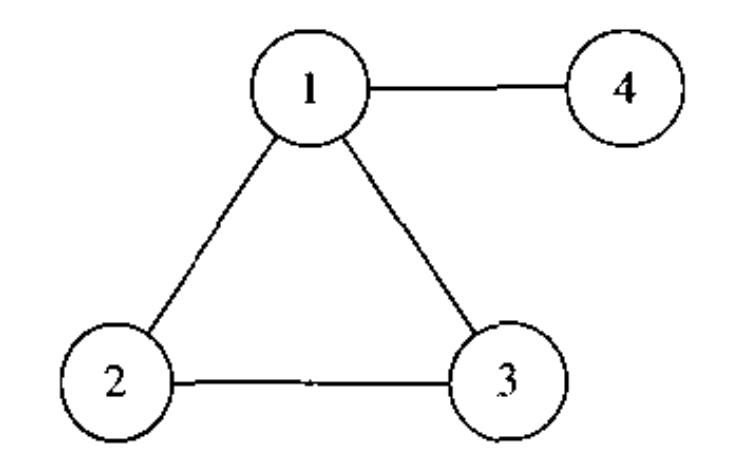
\includegraphics[width=0.3\textwidth]{Comparibility_graph_mux}
    \caption{ Compatibility graph \cite{b1}}
    \label{fig:Comparibility_graph_mux}
\end{figure}

\ref{fig:Comparibility_graph_mux_2}
\begin{figure}[h]
    \centering
    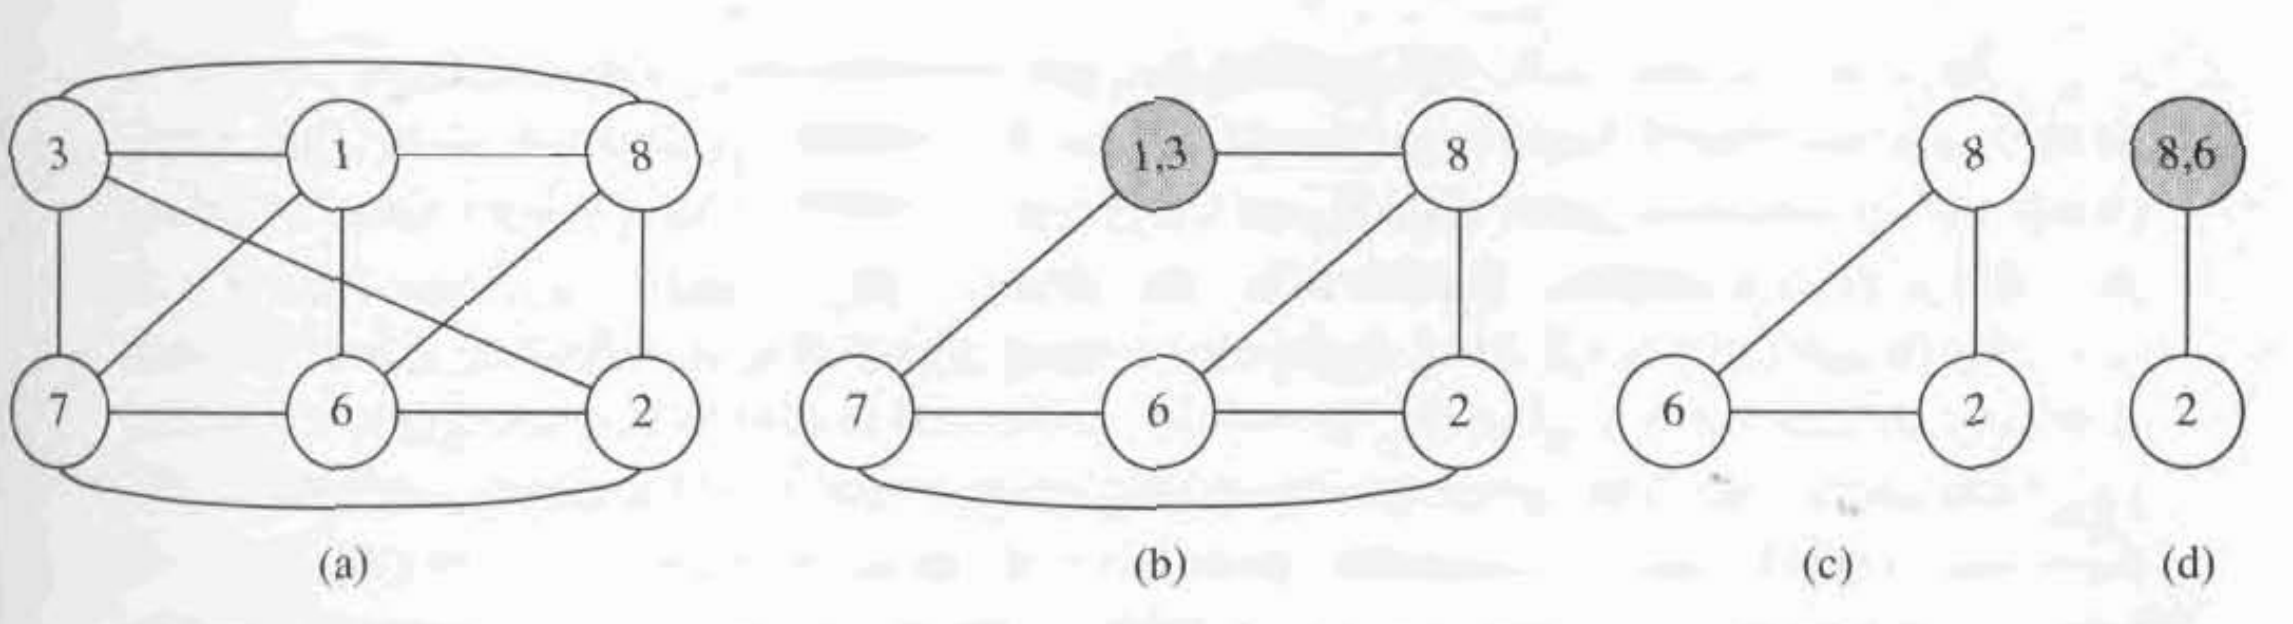
\includegraphics[width=0.5\textwidth]{Comparibility_graph_mux_2}
    \caption{ (a) Compatibility graph for the multiplier type. (b) Reduced compatibility graph with clique seed. (c) Fragment of compatibility graph after one clique has heen removed. (d) Reduced fragment with clique seed. \cite{b1}}
    \label{fig:Comparibility_graph_mux_2}
\end{figure}